\documentclass[12pt,letterpaper]{article}
\usepackage[utf8]{inputenc}
\usepackage[spanish]{babel}
\usepackage{graphicx}
\usepackage[left=2cm,right=2cm,top=2cm,bottom=2cm]{geometry}
\usepackage{graphicx} % figuras
% \usepackage{subfigure} % subfiguras
\usepackage{float} % para usar [H]
\usepackage{amsmath}
%\usepackage{txfonts}
\usepackage{stackrel} 
\usepackage{multirow}
\usepackage{enumerate} % enumerados
\renewcommand{\labelitemi}{$-$}
\renewcommand{\labelitemii}{$\cdot$}
% \author{}
% \title{Caratula}
\begin{document}

% Fancy Header and Footer
% \usepackage{fancyhdr}
% \pagestyle{fancy}
% \cfoot{}
% \rfoot{\thepage}
%

% \usepackage[hidelinks]{hyperref} % CREA HYPERVINCULOS EN INDICE

% \author{}
\title{Caratula}

\begin{titlepage}
\begin{center}
\large{UNIVERSIDAD PRIVADA DE TACNA}\\
\vspace*{-0.025in}
\begin{figure}[htb]
\begin{center}

\includegraphics[width=7cm]{./images/logo}
\end{center}
\end{figure}
\vspace*{0.15in}
INGENIERIA DE SISTEMAS  \\

\vspace*{0.3in}
\begin{large}
\textbf{TITULO:} \\
\end{large}

\vspace*{0.1in}
\begin{Large}
\textbf{Informe de Laboratorio 01: Ejercicio 1: Gestión de casos, conjuntos y planes de prueba} \\

\end{Large}

\vspace*{0.3in}
\begin{Large}
\textbf{CURSO:} \\
\end{Large}

\vspace*{0.1in}
\begin{large}
Calidad y Pruebas de Software\\
\end{large}

\vspace*{0.3in}
\begin{Large}
\textbf{DOCENTE:} \\
\end{Large}

\vspace*{0.1in}
\begin{large}
 Ing. Patrick Cuadros Quiroga\\
\end{large}

\vspace*{0.4in}
\vspace*{0.1in}
\begin{large}
\textbf{INTEGRANTES:} \\
\begin{flushleft}
Katerin Almendra Merino Quispe \hfill	(2018060918)\\

\centering  %CENTRA UN TEXTO
\vspace*{0.9in}
\begin{large}
Tacna
\end{large}

\end{flushleft}
\end{large}
\end{center}

\end{titlepage}


\tableofcontents % INDICE
\thispagestyle{empty} % INDICE SIN NUMERO
\newpage
\setcounter{page}{1} % REINICIAR CONTADOR DE PAGINAS DESPUES DEL INDICE


\section{Tarea 1: Comprensión de casos, conjuntos y planes de prueba} 
\begin{itemize}
 \item  Seleccione Test Plans para navegar hasta Test Hub . El centro de pruebas proporciona un lugar central para toda la planificación, ejecución y análisis de pruebas.
\begin{center}
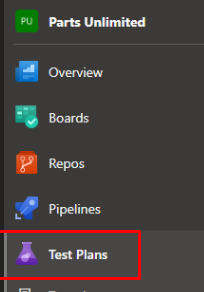
\includegraphics[width=\columnwidth]{images/40}\newline
\end{center}
 \item  En general, cada hito importante de un proyecto debe tener su propio plan de prueba . Dentro de cada plan de prueba hay conjuntos de pruebas , que son conjuntos de casos de prueba (y, opcionalmente, otros conjuntos de pruebas) diseñados para validar un elemento de trabajo, como la implementacion de una función o la corrección de errores. Cada caso de prueba está diseñado para confirmar un comportamiento específico y puede pertenecer a uno o más conjuntos de pruebas. 

\begin{center}
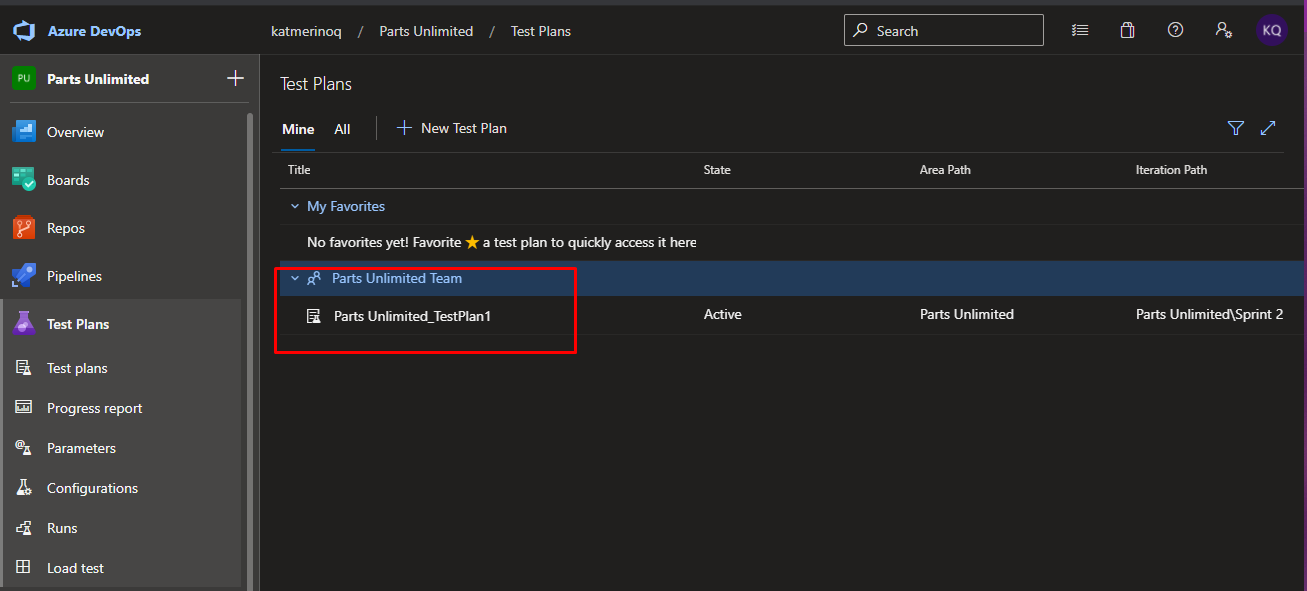
\includegraphics[width=\columnwidth]{images/8}\newline
\end{center}
 
 \item Seleccione el conjunto de pruebas para la historia. Como cliente, me gustaría almacenar los datos de mi tarjeta de crédito de forma segura . Este conjunto de pruebas se centra en ese elemento de trabajo, que resulta ser una función. Tenga en cuenta que los números de los elementos de trabajo variarán cada vez que genere datos de demostración para un laboratorio.
\begin{center}
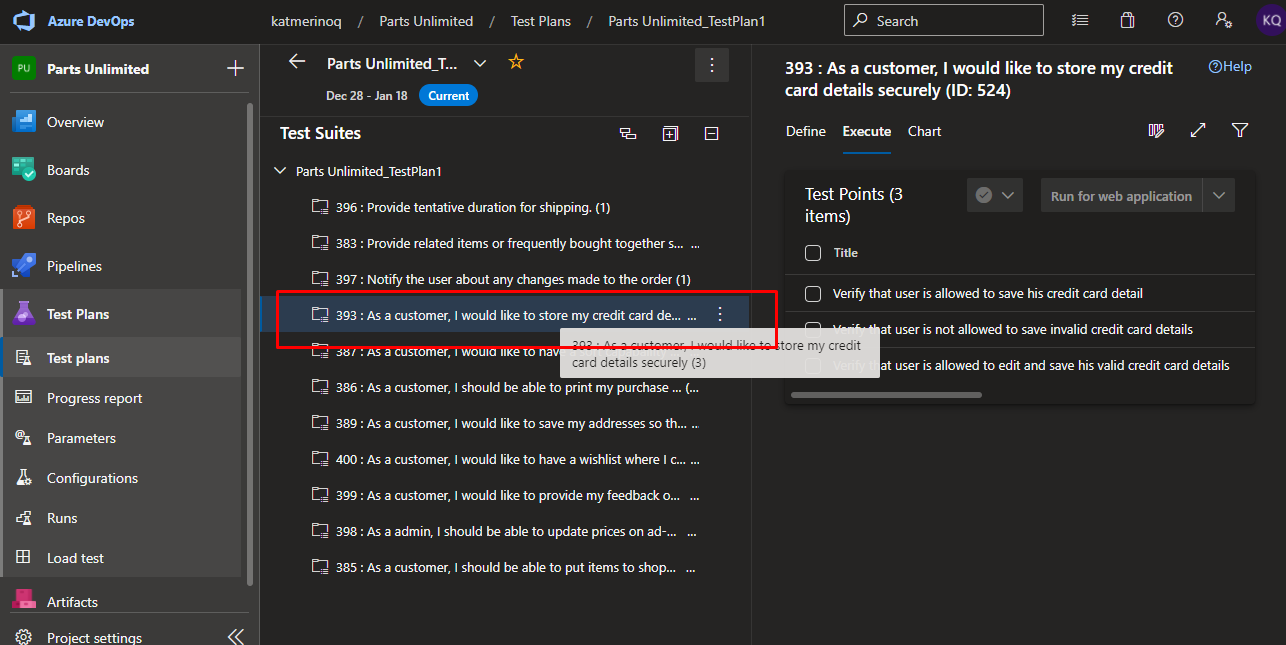
\includegraphics[width=\columnwidth]{images/9}\newline
\end{center}

\item En el lado derecho, puede ver que este conjunto de pruebas tiene tres casos de prueba diseñados para confirmar el comportamiento esperado de la implementación de la función. Haga doble clic en Verificar que el usuario pueda guardar el caso de prueba de detalles de su tarjeta de crédito.
\begin{center}
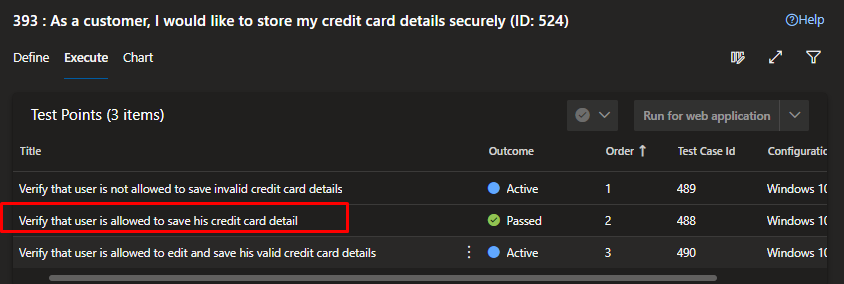
\includegraphics[width=\columnwidth]{images/41}\newline
\end{center}

\item Este cuadro de diálogo proporciona toda la información que necesita sobre este caso de prueba. Busque el panel Trabajo relacionado y tenga en cuenta que este caso de prueba está vinculado a la suite a la que pertenece. Haga clic en el elemento de trabajo para navegar hasta él.
\begin{center}
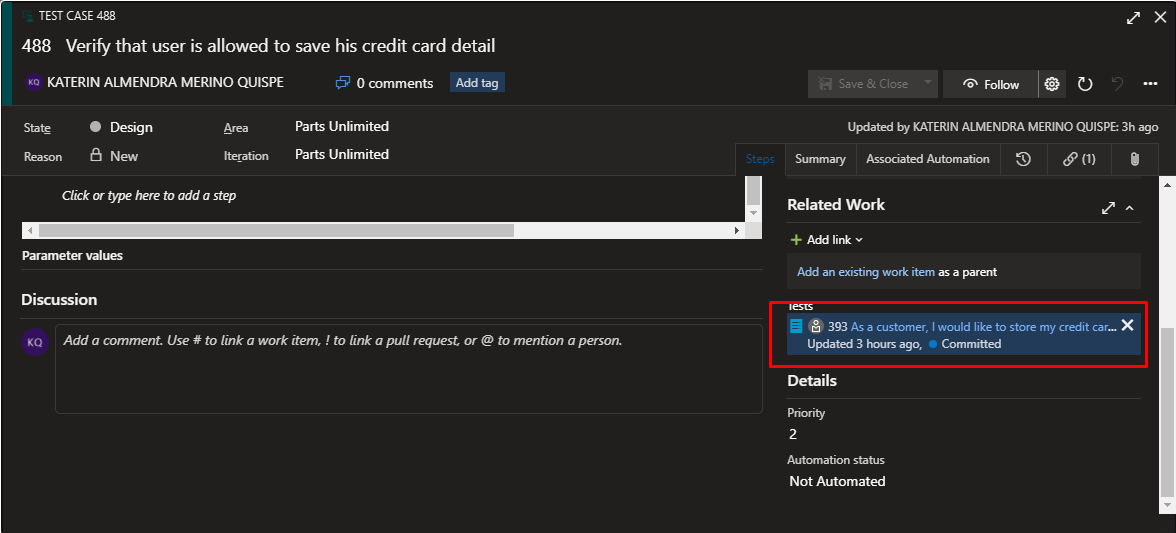
\includegraphics[width=\columnwidth]{images/22}\newline
\end{center} 

\item En el conjunto de pruebas, podemos ver todos los elementos de trabajo vinculados, que resultan ser los casos de prueba.
\begin{center}
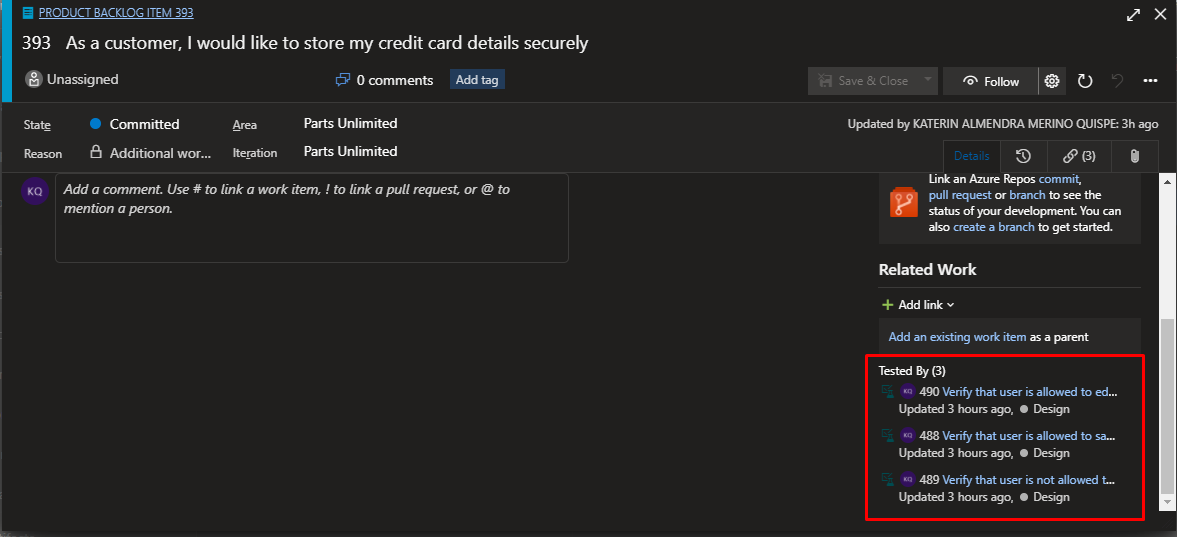
\includegraphics[width=\columnwidth]{images/23}\newline
\end{center}

\item Sin embargo, aún no está asociado con la función para la que está diseñado para probar, que podemos vincular ahora. Haga clic en Agregar enlace | Elemento existente.
\begin{center}
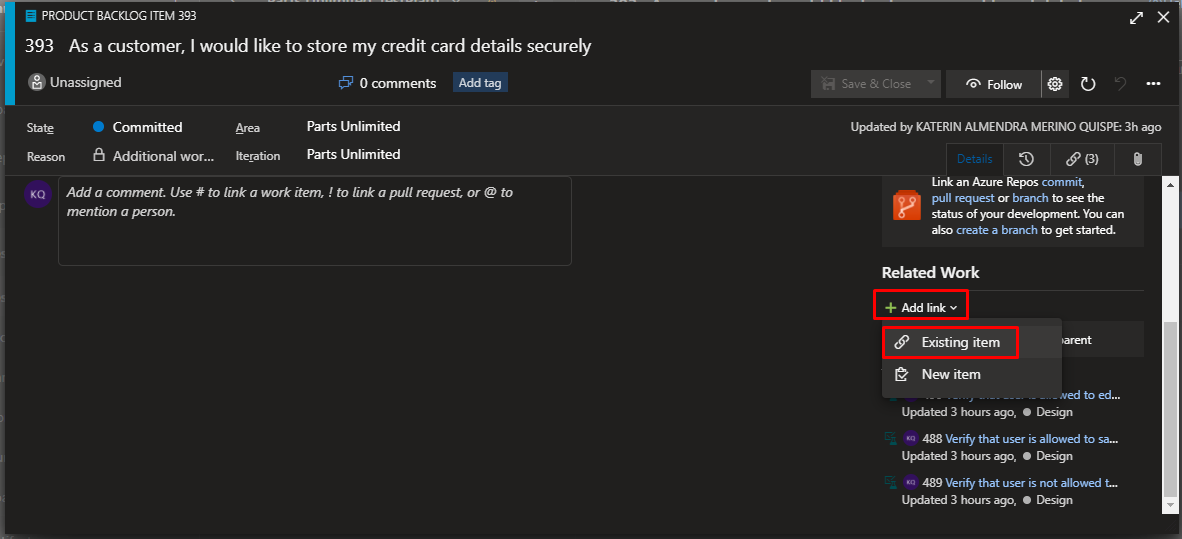
\includegraphics[width=\columnwidth]{images/24}
\end{center} 

\item Establezca el tipo de vínculo en Padre y busque "tarjeta de crédito".
\begin{center}
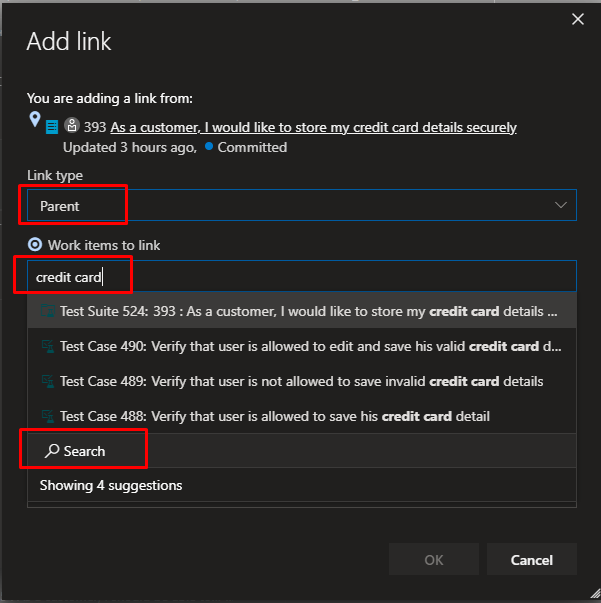
\includegraphics[width=\columnwidth]{images/25}\newline
\end{center}

\item Seleccione la función para compra con tarjeta de crédito.
\item Haga clic en Aceptar.
\begin{center}
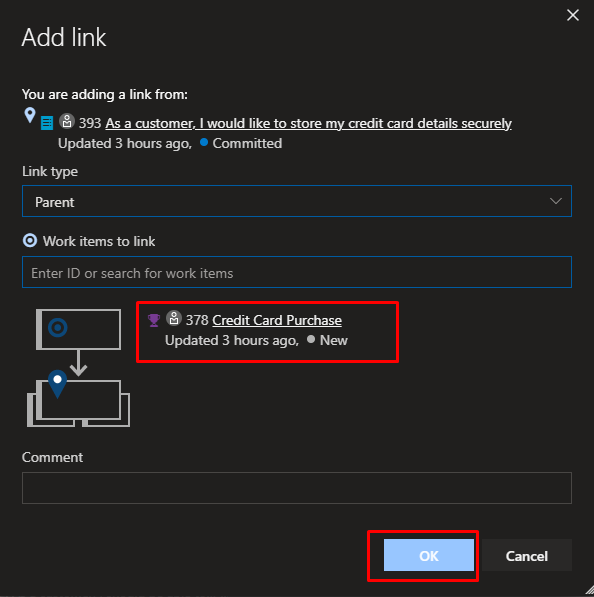
\includegraphics[width=\columnwidth]{images/26}\newline
\end{center}

\item La función principal ahora está asociada con la suite que la prueba y cualquiera puede navegar entre ellos para ver su relación en relación con los otros elementos de trabajo involucrados.
\begin{center}
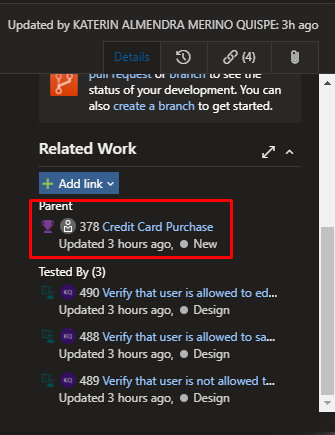
\includegraphics[width=\columnwidth]{images/27}\newline
\end{center}

\item Haga clic en Guardar y cerrar .
\begin{center}
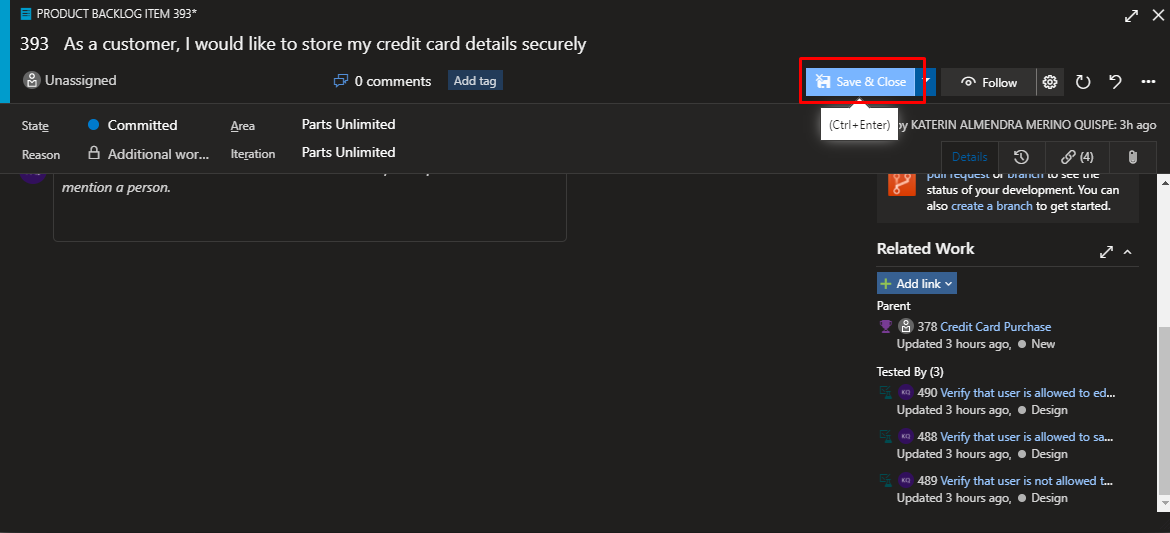
\includegraphics[width=\columnwidth]{images/28}\newline
\end{center}
\end{itemize}

\section{Tarea 2: Gestión de pruebas} 
\begin{itemize}
\item A veces, se debe ejecutar un conjunto de casos de prueba en un orden específico para maximizar la eficiencia. Haga clic en Solicitar pruebas para especificar el orden en que se deben ejecutar estos casos de prueba.
\item Ahora puede ver que el pedido se ha actualizado y que la lista ahora está ordenada por él.
\begin{center}
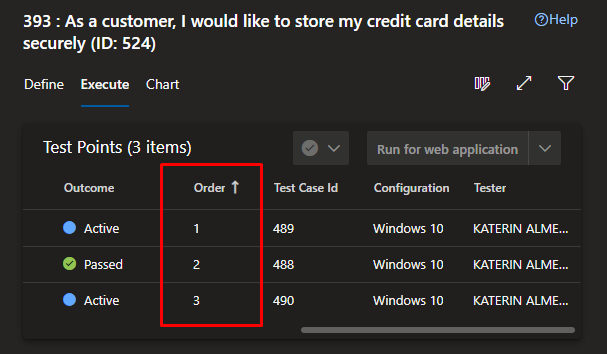
\includegraphics[width=\columnwidth]{images/29}\newline
\end{center}

\item Otro aspecto importante de las pruebas tiene que ver con el entorno en el que se ejecuta cada prueba. Para esta aplicación web, el navegador y el sistema operativo son consideraciones clave. En este momento, todas las pruebas solo usan una configuración: Windows 10.
\begin{center}
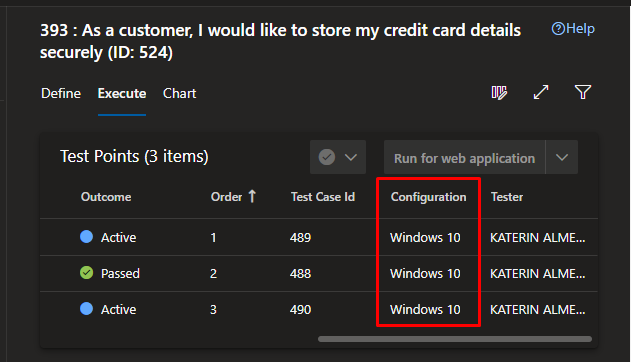
\includegraphics[width=\columnwidth]{images/30}\newline
\end{center}

\item Seleccione la pestaña Configuraciones.
\begin{center}
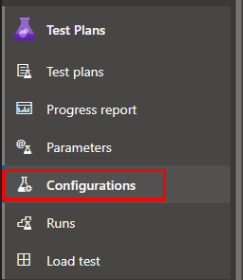
\includegraphics[width=\columnwidth]{images/42}\newline
\end{center}

\item Tenga en cuenta que hay una configuración existente para Windows 10 . Cada configuración de prueba incluye un nombre y una descripción, así como un conjunto de variables de configuración personalizables . Este proyecto tiene una variable de configuración establecida para el sistema operativo . Puede agregar fácilmente más y / o editar las entradas disponibles para cada uno. Haga clic en Agregar variable de configuración.
\item Seleccione la variable del navegador y configúrela en Microsoft Edge.
\item Haga clic en Guardar para guardar la configuración.
\begin{center}
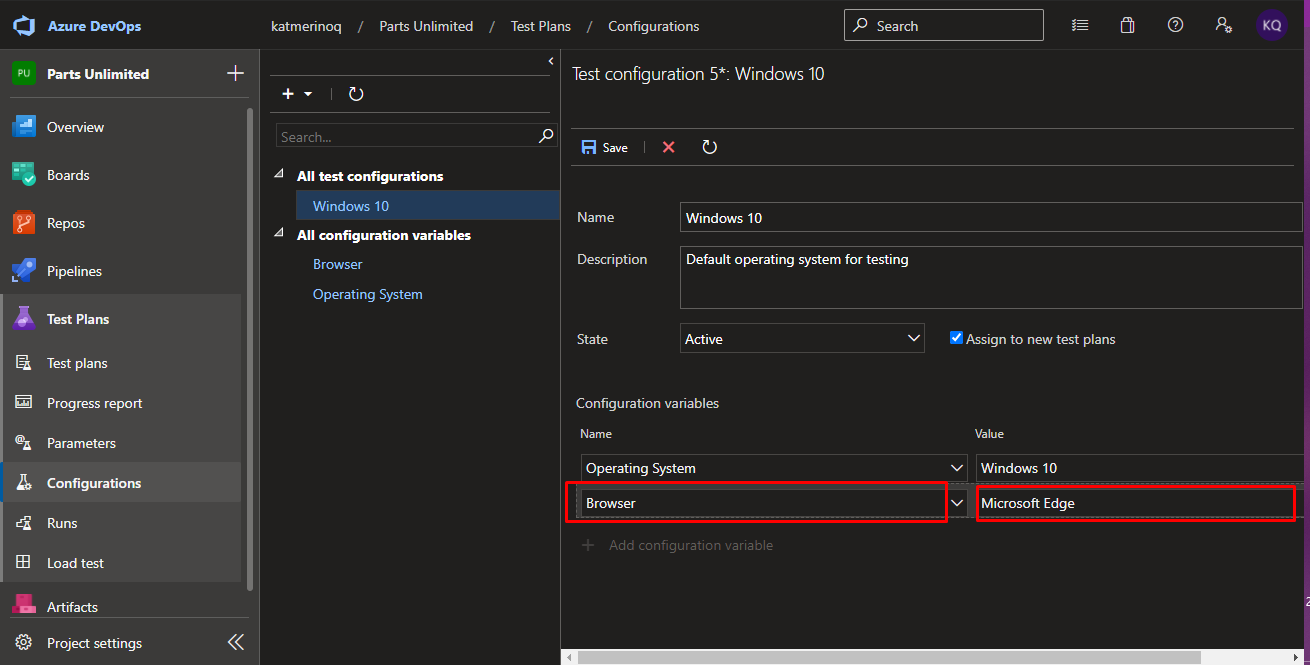
\includegraphics[width=\columnwidth]{images/10}\newline
\end{center}

\item Ahora supongamos que el equipo de prueba ha adquirido un iPhone X y quiere agregarlo a la matriz de prueba. Es realmente fácil registrar este entorno como una nueva configuración para que los casos de prueba puedan especificarlo. Sin embargo, antes de agregarlo, necesitaremos una opción de sistema operativo para iOS 10 . Haga clic en la variable de configuración del sistema operativo.
\begin{center}
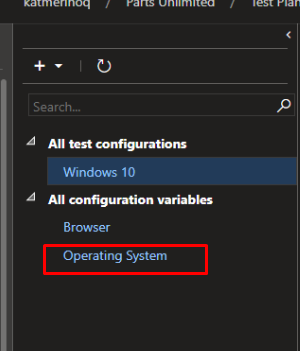
\includegraphics[width=\columnwidth]{images/43}\newline
\end{center}

\item Haga clic en Agregar nuevo valor y agregue una entrada para iOS 12.
\item Haga clic en Guardar .
\begin{center}
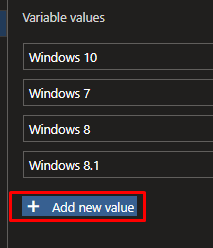
\includegraphics[width=\columnwidth]{images/44}\newline
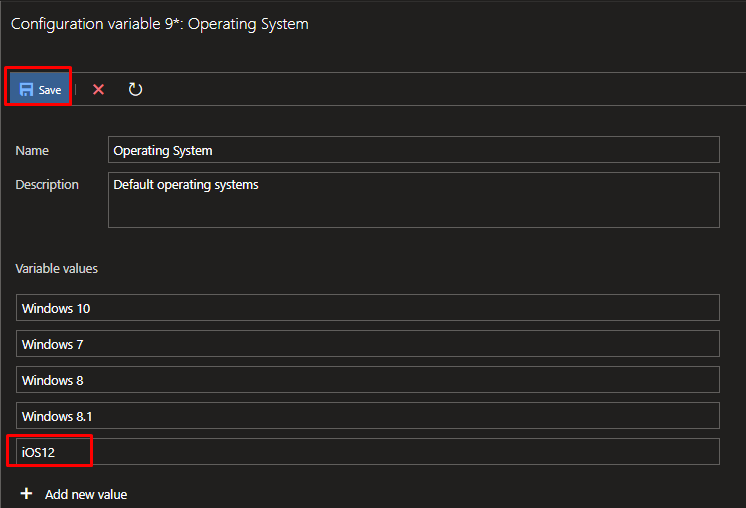
\includegraphics[width=\columnwidth]{images/45}\newline
\end{center}

\item Ahora tenemos todo lo que necesitamos para agregar el iPhone X. Haga clic en el menú desplegable Agregar y seleccione Nueva configuración de prueba.
\begin{center}
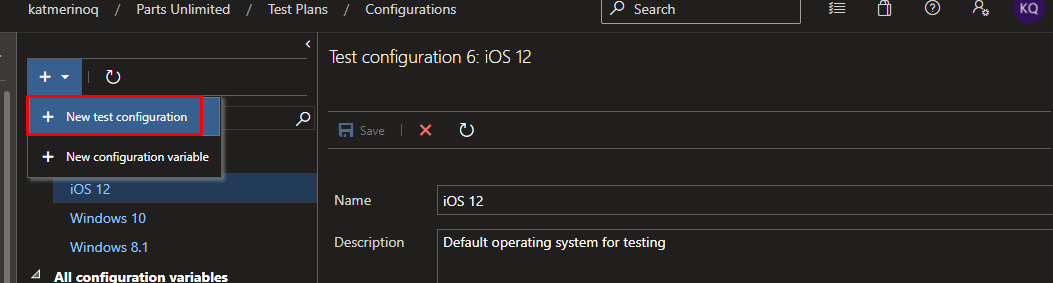
\includegraphics[width=\columnwidth]{images/11}\newline
\end{center}

\item Establezca el nombre en "iPhone X".
\item Haga clic en Agregar variable de configuración dos veces y configure el navegador en Safari y el sistema operativo en iOS 12.
\item Haga clic en Guardar para guardar la nueva configuración.
\begin{center}
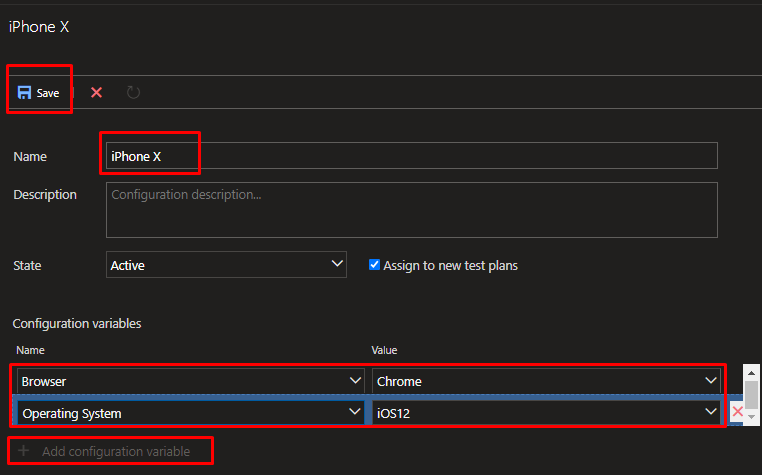
\includegraphics[width=\columnwidth]{images/46}\newline
\end{center}

\item Regrese a la pestaña Planes de prueba.
\item Haga clic en el menú desplegable junto al conjunto de pruebas con el que hemos estado trabajando hasta ahora y seleccione Asignar configuraciones al conjunto de pruebas.
\begin{center}
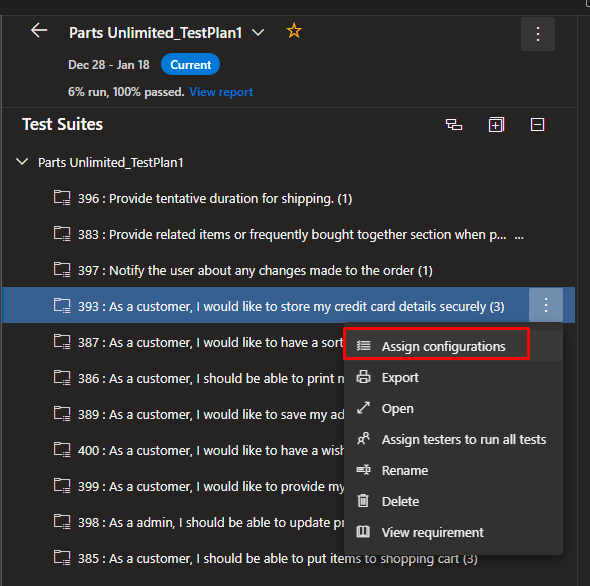
\includegraphics[width=\columnwidth]{images/13}\newline
\end{center}

\item Marque la opción iPhone X y haga clic en Guardar.
\begin{center}
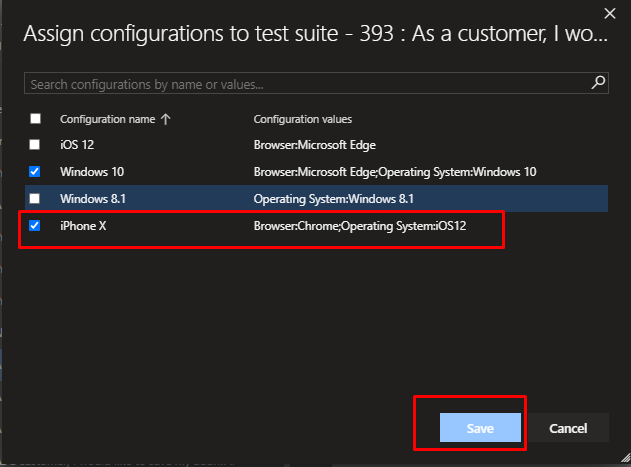
\includegraphics[width=\columnwidth]{images/47}\newline
\end{center}

\item Tenga en cuenta que cada caso de prueba se ha duplicado con una configuración adicional para iPhone X . Ahora cada entorno se puede probar y rastrear por separado.
\begin{center}
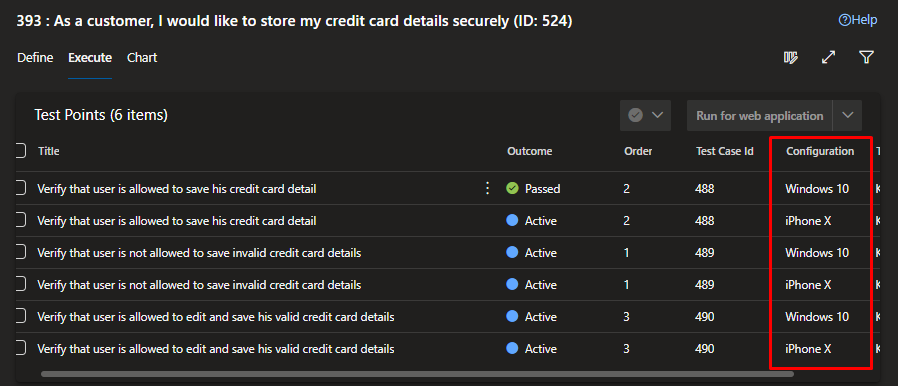
\includegraphics[width=\columnwidth]{images/48}\newline
\end{center}
\end{itemize}

\section{Tarea 3: Autoría de pruebas} 

\begin{itemize}

\item Expanda el menú desplegable junto al plan de prueba y seleccione Nueva suite estática. Un conjunto estático de casos de prueba es un conjunto donde los casos se han asignado manualmente. También puede crear suites basado en requisitos comunes ( baño a base de requerimiento ) o una consulta de casos de prueba y / o elementos de trabajo ( privado basado en consultas ).
\begin{center}
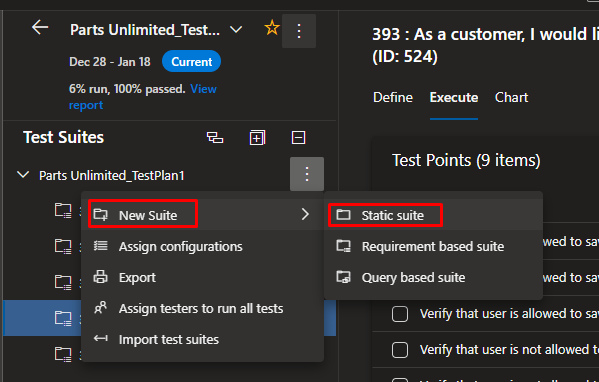
\includegraphics[width=\columnwidth]{images/16}\newline
\end{center}

\item Establezca el nombre de la nueva suite en "Pruebas de envío" . Todas estas pruebas se centrarán en la funcionalidad relacionada con el envío. Recuerde que puede compartir fácilmente casos de prueba entre suites, por lo que hay una redundancia mínima cuando hay muchas suites superpuestas.
\begin{center}
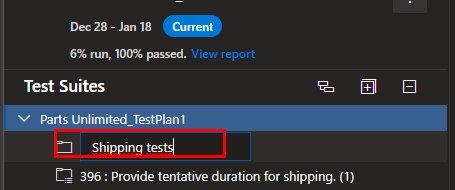
\includegraphics[width=\columnwidth]{images/17}\newline
\end{center}

\item Expanda el menú desplegable junto al paquete recién creado y seleccione Nuevo paquete basado en requisitos.
\begin{center}
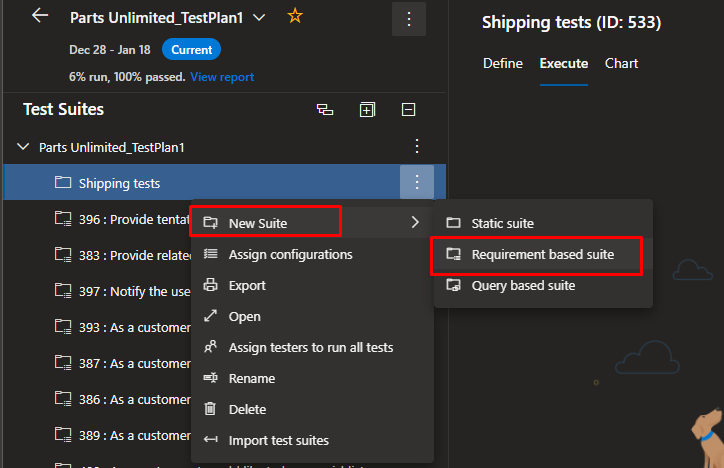
\includegraphics[width=\columnwidth]{images/18}\newline
\end{center}

\item Puede personalizar la consulta utilizada para especificar qué requisitos se recuperan, pero deje los valores predeterminados y haga clic en Ejecutar consulta . Busque y seleccione los tres elementos de la cartera de productos relacionados con el envío. Haga clic en Crear conjuntos para crear un conjunto de pruebas para cada uno.
\begin{center}
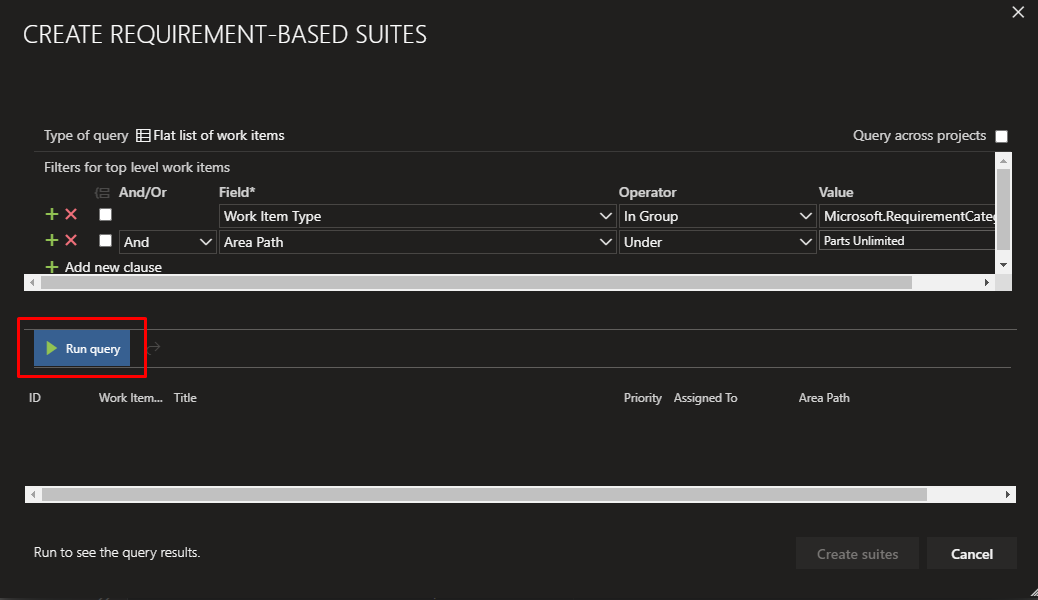
\includegraphics[width=\columnwidth]{images/19}\newline
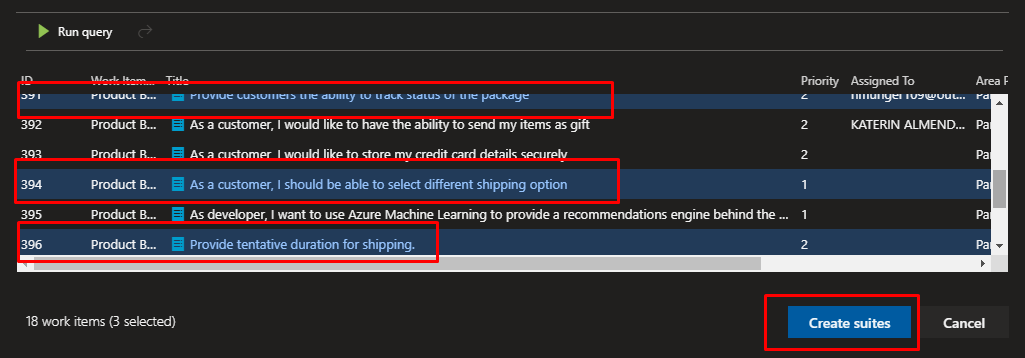
\includegraphics[width=\columnwidth]{images/20}\newline
\end{center}

\item Seleccione una de las suites recién creadas, como la asociada con el seguimiento del estado del paquete.
\item Si bien puede crear casos de prueba uno a la vez, a veces es más fácil usar un diseño de cuadrícula para agregar rápidamente muchos casos de prueba. En el panel de casos de prueba, seleccione Nuevo | Nuevo caso de prueba usando grid.
\begin{center}
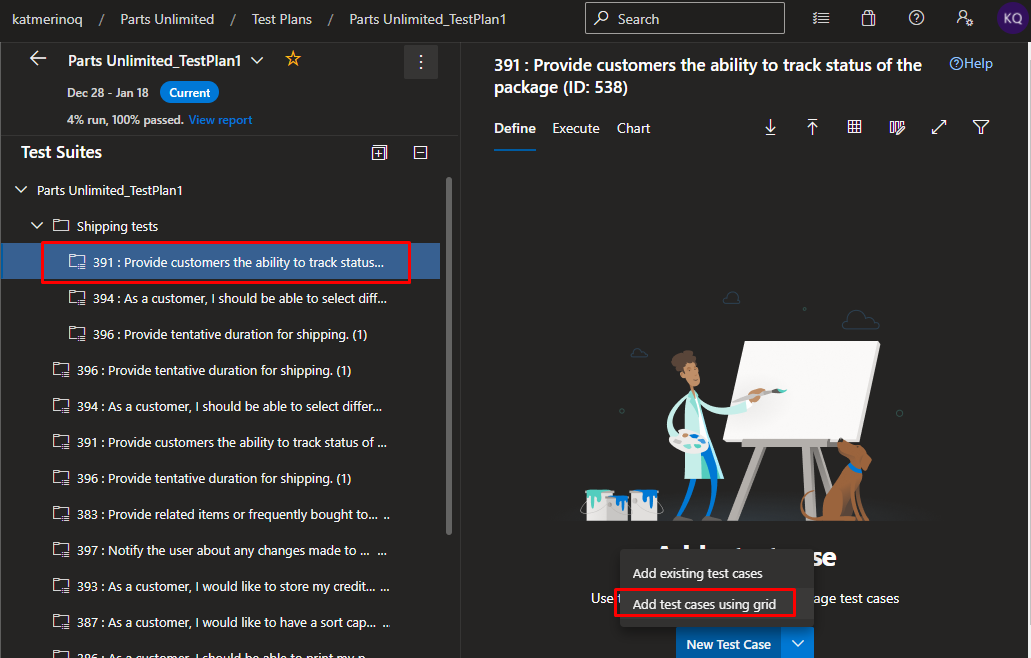
\includegraphics[width=\columnwidth]{images/33}\newline
\end{center}

\item Ingrese algunos casos de prueba y haga clic en el botón Guardar todo . El título será el título eventual del caso de prueba. Paso La acción será el primer paso (y posiblemente el único) de la prueba. Si ese paso tiene un resultado esperado, puede especificarlo como Resultado esperado del paso.
\begin{center}
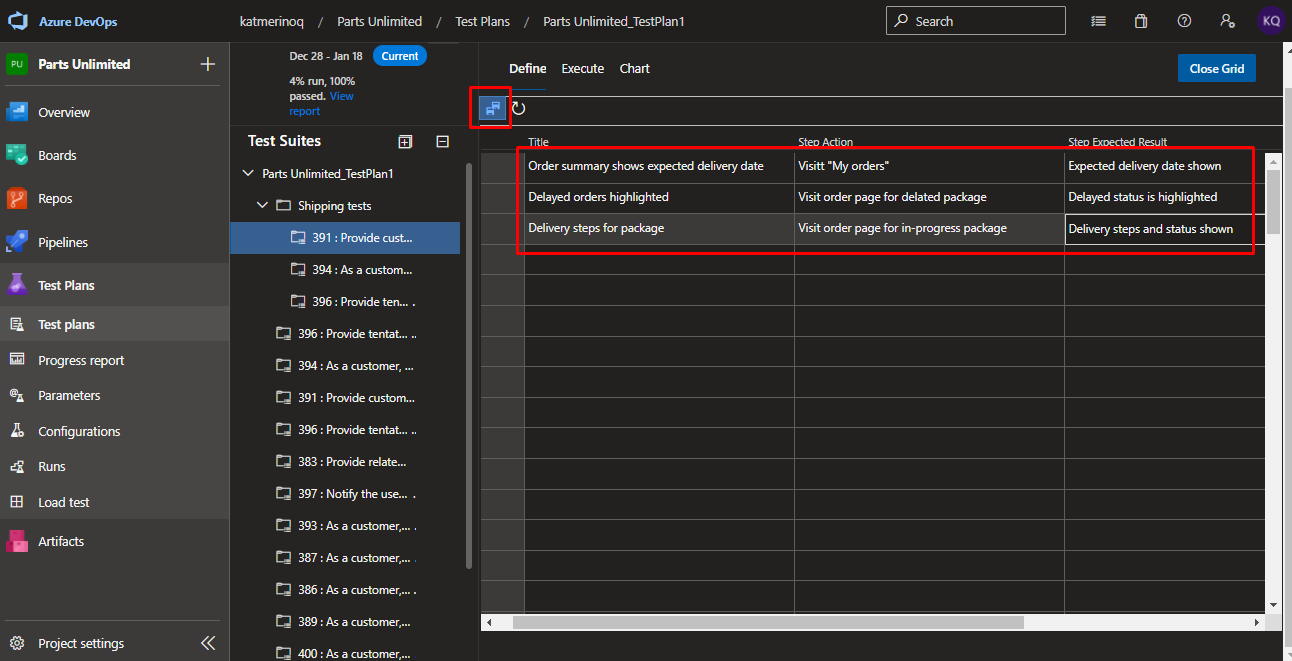
\includegraphics[width=\columnwidth]{images/34}\newline
\end{center}

\item Opcionalmente, puede continuar agregando y editando elementos de trabajo en la vista de cuadrícula. Cuando esté satisfecho, vuelva a la vista de lista haciendo clic en el botón Ver: Cuadrícula.
\begin{center}
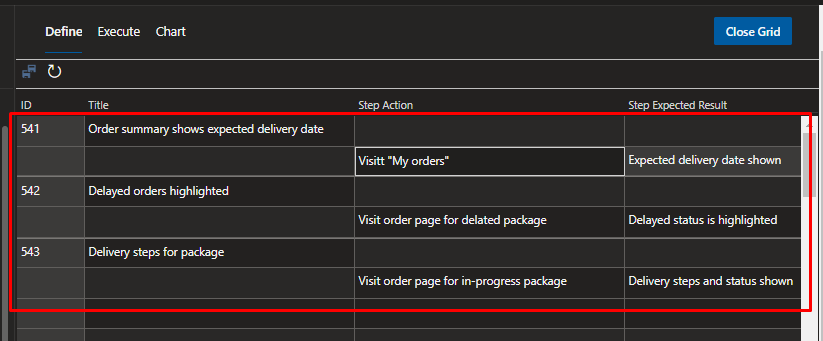
\includegraphics[width=\columnwidth]{images/35}\newline
\end{center}

\item La vista de lista muestra los mismos datos, pero en una vista diferente.
\begin{center}
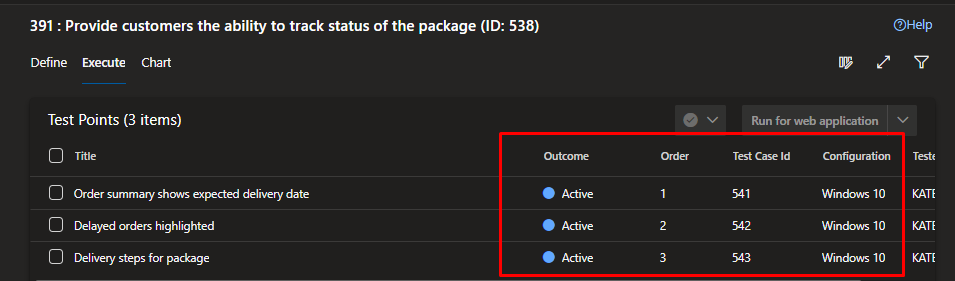
\includegraphics[width=\columnwidth]{images/36}\newline
\end{center}

\item Otra opción para crear conjuntos es mediante la consulta de elementos de trabajo. Expanda el menú desplegable junto al paquete de pruebas de envío y seleccione un nuevo paquete basado en consultas.
\begin{center}
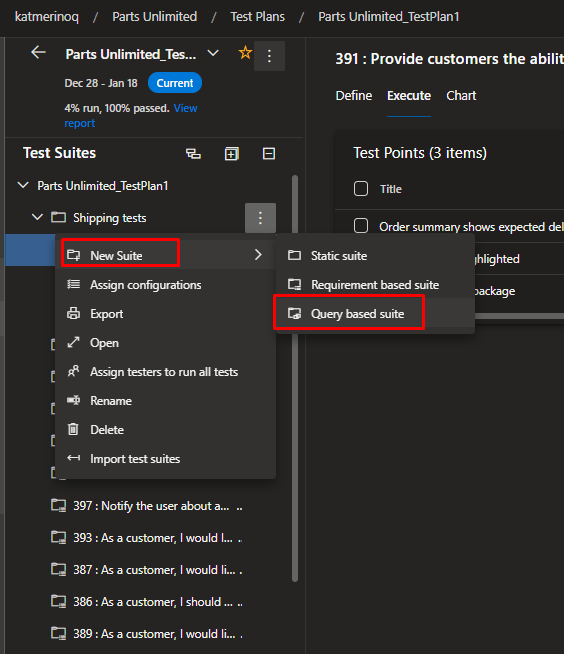
\includegraphics[width=\columnwidth]{images/37}\newline
\end{center}

\item Otra opción para crear conjuntos es mediante la consulta de elementos de trabajo. Expanda el menú desplegable junto al paquete de pruebas de envío y seleccione un nuevo paquete basado en consultas.Supongamos que desea crear un conjunto de pruebas a partir de casos de prueba relacionados con el envío en el proyecto. Cambie el Tipo de elemento de trabajo a Microsoft.TestCaseCategory para buscar casos de prueba y haga clic en Ejecutar consulta . Ahora tiene una lista de casos de prueba que puede seleccionar para crear conjuntos, si lo desea.
\begin{center}
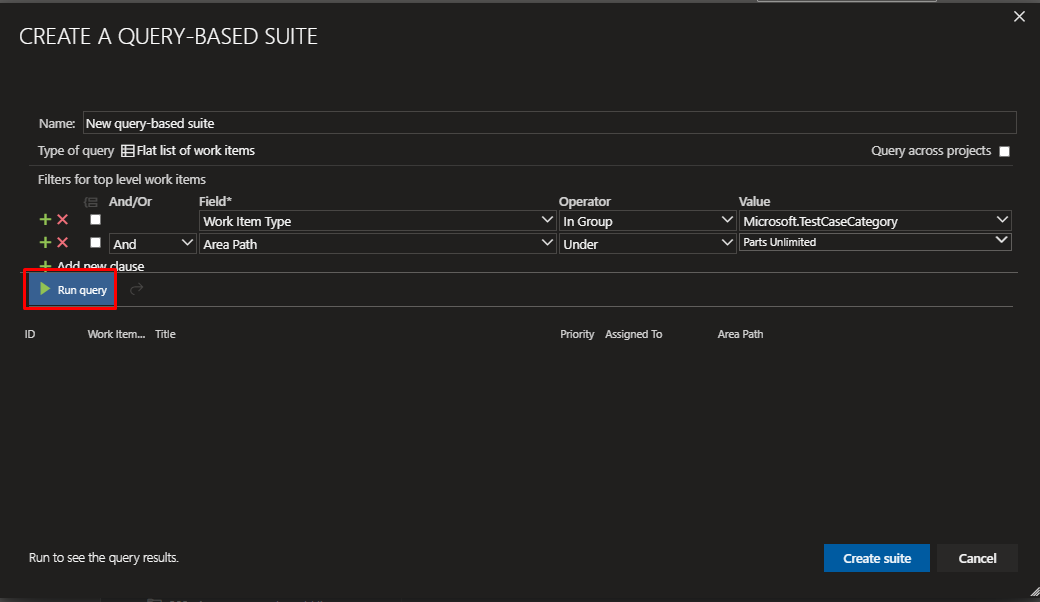
\includegraphics[width=\columnwidth]{images/38}\newline
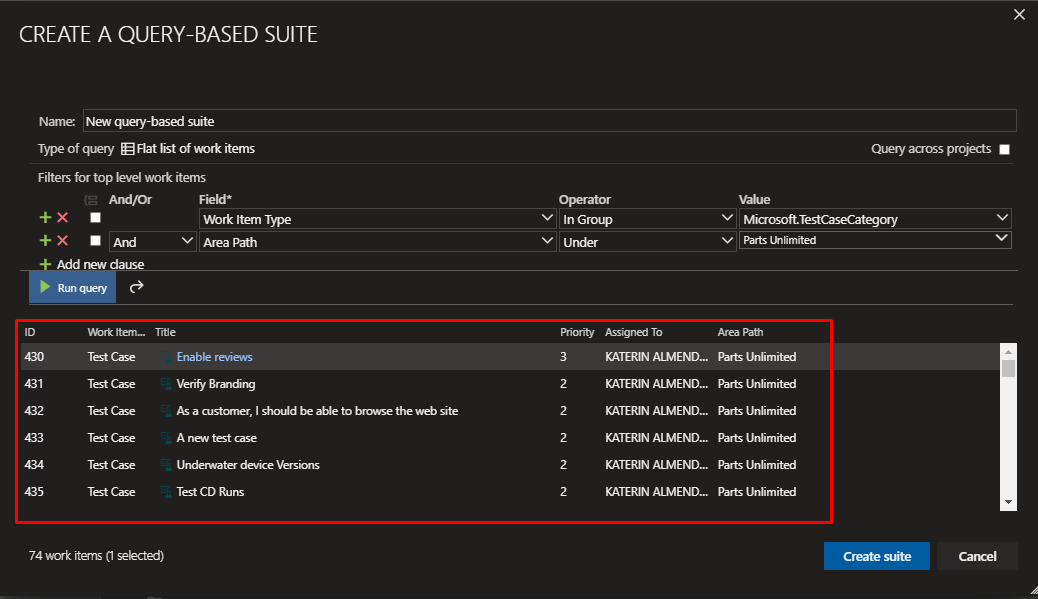
\includegraphics[width=\columnwidth]{images/39}\newline
\end{center}

\item Presione Esc para cerrar el diálogo
\end{itemize}





\end{document}